% chktex-file 44 32 36 38 18 11 8 26


\medskip

\exods{\getpts{Exo2}}
%AN1J2 exo3

\section*{PARTIE A}

Dans cette partie, on pourra utiliser les clauses du langage SQL pour:

\begin{itemize}
    \item construire des requêtes d'interrogation à l'aide de \texttt{SELECT}, \texttt{FROM}, \texttt{WHERE} (avec les opérateurs logiques \texttt{AND}, \texttt{OR}), \texttt{JOIN\ldots{} ON};
    \item construire des requêtes d'insertion et de mise à jour à l'aide de \texttt{UPDATE}, \texttt{INSERT}, \texttt{DELETE};
    \item affiner les recherches à l'aide de \texttt{DISTINCT}, \texttt{ORDER BY}.
\end{itemize}

La compagnie aérienne AirInfo souhaite utiliser un système de gestion de bases de données relationnelles afin de l'aider à gérer les informations dont elle dispose sur les aéroports desservis, les vols proposés, les passagers et les réservations effectuées par ces passagers.

Elle crée donc la base de données \texttt{compagnie\_aerienne}, constituée de quatre relations. Le schéma relationnel de cette base de données est le suivant:

\begin{lstlisting}[language=SQL, numbers=none]
aeroport(id_aeroport : TEXT, ville : TEXT, pays : TEXT)
vol(id_vol : TEXT, aeroport_dep : TEXT, aeroport_arr : TEXT, dist : INT)
passager(id_passager : INT, nom : TEXT, ville : TEXT, d_totale : INT)
reservation(id_vol : TEXT, id_passager : INT)
\end{lstlisting}

Une clé primaire de la relation vol est l'attribut \texttt{id\_vol}. Les autres clés primaires et étrangères ne sont pas précisées.

Les quatre tables de l'\textbf{annexe 2} constituent, en l'état, la base de données \texttt{compagnie\_aerienne} complète.

Les valeurs des champs \texttt{distance} et \texttt{d\_totale} intervenant respectivement dans les tables \texttt{vol} et \texttt{passager} sont exprimées en milliers de kilomètres.

\medskip
\begin{center}
\textbf{ANNEXE 2}
\end{center}
\medskip



\begin{enumerate}[resume=monDS]
    \item  Expliquer pourquoi l'attribut \texttt{id\_vol} ne peut pas être une clé primaire de la table \texttt{reservation}. (/\getpts{Q11})
\begin{blocvisiblex}[height=3]
    {\quad}
    L'attribut \texttt{id\_vol} ne peut pas être une clé primaire de la table \texttt{reservation} car il peut y avoir plusieurs réservations pour un même vol, comme le montre la table \texttt{reservation} où le vol AI0006 est réservé par deux passagers différents (\texttt{id\_passager} 1 et 2). Par conséquent, l'attribut \texttt{id\_vol} ne permet pas d'identifier de manière unique chaque enregistrement de la table \texttt{reservation}.
\end{blocvisiblex}

\item Proposer une clé primaire pour la table \texttt{reservation}. (/\getpts{Q12})
\begin{blocvisiblex}[height=3]
    {\quad}
    Une clé primaire pour la table \texttt{reservation} pourrait être la combinaison des attributs \texttt{id\_vol} et \texttt{id\_passager}. En effet, cette combinaison permettrait d'identifier de manière unique chaque enregistrement de la table, car un même vol peut être réservé par plusieurs passagers, mais un même passager ne peut pas réserver le même vol plus d'une fois.
\end{blocvisiblex}
\item Expliquer le rôle d’une clé étrangère dans une relation. (/\getpts{Q13})
\begin{blocvisiblex}[height=3]
    {\quad}
    Une clé étrangère dans une relation est un attribut ou un ensemble d'attributs qui fait référence à la clé primaire d'une autre relation. Son rôle est de créer un lien entre les deux relations, permettant ainsi d'assurer l'intégrité référentielle des données. En utilisant des clés étrangères, on peut garantir que les données dans une table sont cohérentes avec les données dans une autre table, et cela facilite également les opérations de jointure entre les tables lors de l'interrogation de la base de données.
\end{blocvisiblex}
\item Écrire le résultat renvoyé par la requête SQL suivante: (/\getpts{Q14})
\begin{lstlisting}[language=SQL]
SELECT id_vol 
FROM vol 
WHERE aeroport_arr = 'CDG'
\end{lstlisting}

\begin{blocvisible}[height=3]
        Le résultat renvoyé par la requête SQL serait une liste des \texttt{id\_vol} des vols dont l'aéroport d'arrivée est \verb|'CDG'|. En se basant sur la table \texttt{vol}, les vols correspondants seraient AI0015, AI0258, AI0292.
\end{blocvisible}

\medskip



\item Écrire une requête SQL qui donne les noms des villes qui sont destination d'un vol au départ de l'aéroport CDG\@. (/\getpts{Q15})
\begin{blocvisible}[height=2.5]
\begin{lstlisting}[language=SQL,frame=none, numbers=none]
SELECT aeroport.ville 
FROM aeroport 
JOIN vol ON aeroport.id_aeroport = vol.aeroport_arr
WHERE vol.aeroport_dep = 'CDG';
\end{lstlisting}
\end{blocvisible}



\end{enumerate}


\medskip


La compagnie AirInfo envisage de récompenser la fidélité de ses usagers en tenant compte de la distance totale qu'ils parcourent sur leurs lignes. 


Ainsi, à chaque nouvelle réservation, la table passager doit être mise à jour: si l'usager avait déjà parcouru une distance totale $d_{\texttt{totale}}$, puis réserve un vol d'une distance $d_{\texttt{vol}}$, l'attribut \texttt{d\_totale} est modifié en prenant pour nouvelle valeur $d_{\texttt{totale}} + d_{\texttt{vol}}$.

\begin{enumerate}[resume=monDS]
    \item La passagère d'identifiant 5 a déjà parcouru 10 milliers de kilomètres. Elle réserve un vol de Washington (IAD) à Paris (CDG), d'une distance de 6 milliers de kilomètres.
    
Écrire la requête permettant de mettre à jour la table passager. (/\getpts{Q16})

\begin{blocvisible}[height=2.5]
\begin{lstlisting}[language=SQL,frame=none, numbers=none]
UPDATE passager
SET d_totale = d_totale + 6
WHERE id_passager = 5;
\end{lstlisting}
\end{blocvisible}
\end{enumerate}

\medskip

La compagnie aérienne offre maintenant la possibilité de relier Paris CDG à Montréal YUL (Canada) par un vol de 6 milliers de kilomètres. Afin de prendre en compte ce nouveau trajet dans la base de données, on souhaite l'ajouter dans la table \texttt{vol} dont la clé primaire est \texttt{id\_vol}. On propose, de manière incorrecte, la requête d'insertion ci-après:

\begin{lstlisting}[language=SQL]
INSERT INTO vol VALUES ('AI0256', 'CDG', 'YUL', 6);
\end{lstlisting}

\begin{enumerate}[resume=monDS]
    \item Proposer, en justifiant, une correction relative à l'erreur commise. (/\getpts{Q17})
\begin{blocvisible}[height=3.5]
    La requête d'insertion proposée est incorrecte car elle utilise une valeur d'identifiant de vol ('AI0256') qui existe déjà dans la table \texttt{vol}. En effet, l'identifiant 'AI0256' est déjà utilisé pour le vol de CDG à SYD. Pour corriger cette erreur, il faut choisir un nouvel identifiant de vol qui n'existe pas encore dans la table, par exemple 'AI0257'. La requête corrigée serait donc:
\begin{lstlisting}[language=SQL,frame=none, numbers=none]    
INSERT INTO vol VALUES ('AI0257', 'CDG', 'YUL', 6);
\end{lstlisting}
\end{blocvisible}
\end{enumerate}

\pagebreak
\section*{PARTIE B}

Dans cette partie, on considère les villes suivantes: Washington(W); Paris(P); Berlin(B); Tokyo(T); Sydney(S).

Les distances des vols entre ces villes, exprimées en milliers de kilomètres, sont les suivantes:

\medskip


\begin{minipage}{0.35\linewidth}
    \begin{itemize}
    \item Washington~--~Paris: 6;
    \item Paris~--~Tokyo: 10;
    \item Paris~--~Sydney: 17;
    \item Berlin~--~Tokyo: 9;
    \item Tokyo~--~Sydney: 8.
\end{itemize}
\end{minipage}
\hfill
\begin{minipage}{0.6\linewidth}
    \centering
    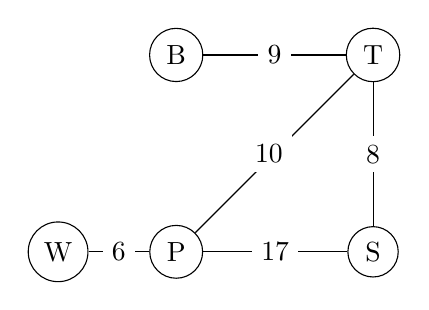
\begin{tikzpicture}[
        node distance={15mm}, 
        main/.style = {draw, circle, minimum size=6mm}
    ] 
        % Définition des nœuds (positionnement relatif)
        \node[main] (W) {W}; 
        \node[main] (P) [right of=W] {P}; 
        \node[main] (S) [right of=P, xshift=1cm] {S}; 
        \node[main] (T) [above of=S, yshift=1cm] {T};
        \node[main] (B) [left of=T, xshift=-1cm] {B};

        % Définition des arêtes avec les pondérations
        \draw (W) -- node[midway, fill=white] {6} (P);
        \draw (P) -- node[midway, fill=white] {17} (S);
        \draw (S) -- node[midway, fill=white] {8} (T);
        \draw (T) -- node[midway, fill=white] {9} (B);
        \draw (P) -- node[midway, fill=white, xshift=-2pt] {10} (T);
        
    \end{tikzpicture}
    \captionof{figure}{Graphe du réseau aérien}\label{reseau_aerien}

\end{minipage}

\medskip

La compagnie AirInfo propose certains de ces vols. Son réseau aérien est représenté par le graphe pondéré non orienté de la figure suivante dans lequel:
\begin{itemize}
    \item chaque ville est représentée par un sommet;
    \item chaque vol direct entre deux villes est représenté par une arête.
\end{itemize}
Le nombre indiqué sur chaque arête est appelé poids: il représente la distance entre deux villes. Cette distance est la même dans un sens ou dans l'autre.

\smallskip

On choisit de représenter ce graphe en Python à l'aide d'un dictionnaire dans lequel chaque clé est un sommet du graphe et la valeur associée à cette clé est elle-même un dictionnaire, dont les clés sont les villes voisines et les valeurs sont les distances correspondantes.


Le dictionnaire associé au graphe, représenté par la figure précédente, est donné ci-après.

\begin{CodePythontexAlt}[TaillePolice=\large, Largeur=1\linewidth,Centre,Lignes=true,PremLigne=1]{}
graphe_airinfo = {     
    'W': {'P': 6}, 
    'P': {'W': 6, 'T': 10, 'S': 17}, 
    'B': {'T': 9}, 
    'T': {'B': 9, 'P': 10, 'S': 8}, 
    'S': {'P': 17, 'T': 8}     }
    \end{CodePythontexAlt}

\begin{enumerate}[resume=monDS]
    \begin{minipage}{0.69\linewidth}
            \item Déterminer la valeur de l'expression \verb|graphe_airinfo['T']['P']|. (/\getpts{Q18})

    \end{minipage}\hfill
    \begin{minipage}{0.29\linewidth}
    \begin{blocvisible}[height=1]
     10
\end{blocvisible}
        \end{minipage}
\item Écrire le code d'une fonction Python \texttt{vol\_direct} permettant de déterminer s'il existe une liaison directe entre deux villes. Cette fonction prend en paramètres un dictionnaire \texttt{graphe} représentant le graphe, et deux clés du dictionnaire \texttt{ville1} et \texttt{ville2} représentant deux villes, et renvoie \texttt{True} si une telle liaison entre les villes \texttt{ville1} et \texttt{ville2} existe, c'est-à-dire si les deux sommets \texttt{ville1} et \texttt{ville2} sont reliés dans le graphe graphe par une arête, \texttt{False} sinon. Exemples: (/\getpts{Q19})
    \begin{CodePythontexAlt}[TaillePolice=\large, Largeur=1\linewidth,Centre,Lignes=true,PremLigne=1]{}
>>> vol_direct(graphe_airinfo, 'T', 'B') 
True 
>>> vol_direct(graphe_airinfo, 'W', 'B') 
False
    \end{CodePythontexAlt}

\begin{blocvisible}[height=3.5]
\begin{CodePythontexAlt}[TaillePolice=\large, Largeur=1\linewidth,Centre,Lignes=true,PremLigne=1]{}
def vol_direct(graphe, ville1, ville2):
    return ville2 in graphe[ville1].keys()
\end{CodePythontexAlt}
\end{blocvisible}


\end{enumerate}

Afin de limiter leurs empreintes carbone, les voyageurs demandent fréquemment aux compagnies aériennes de déterminer, à partir d'une ville donnée, la liste des villes qu'il est possible d'atteindre par un vol direct tout en ne dépassant pas une certaine distance.

\begin{enumerate}[resume=monDS]
    \item Écrire le code d'une fonction Python \texttt{liste\_villes\_proches} qui permet de répondre à la demande des voyageurs. Cette fonction prend en paramètres un dictionnaire \texttt{graphe} représentant le graphe, une clé du dictionnaire \texttt{ville} et un entier \texttt{d\_max} représentant une distance et renvoie la liste des villes reliées à \texttt{ville} par une arête dans \texttt{graphe} dont le poids est au plus égal à \texttt{d\_max}. Exemples: (/\getpts{Q20})
        \begin{CodePythontexAlt}[TaillePolice=\large, Largeur=1\linewidth,Centre,Lignes=true,PremLigne=1]{}
>>> liste_villes_proches(graphe_airinfo, 'T', 7) 
[ ] 
>>> liste_villes_proches(graphe_airinfo, 'T', 9) 
['B', 'S']

    \end{CodePythontexAlt}
\begin{blocvisible}[height=4.5]
\begin{CodePythontexAlt}[TaillePolice=\large, Largeur=1\linewidth,Centre,Lignes=true,PremLigne=1]{}
def liste_villes_proches(graphe, ville, d_max):
    liste = [ ]
    for ville_voisine, distance in graphe[ville].items():
        if distance <= d_max:
            liste.append(ville_voisine)
    return liste
\end{CodePythontexAlt}
\end{blocvisible}
\end{enumerate}



\medskip

La compagnie aérienne Droidevant, concurrente de la compagnie AirInfo, assure des liaisons différentes. Son réseau aérien peut également être représenté par un graphe dont le dictionnaire correspondant en Python est donné ci-après.

\begin{enumerate}[resume=monDS]
    \item Dessiner, en indiquant le poids sur chaque arête, le graphe représentant le réseau aérien de la compagnie Droidevant. (/\getpts{Q21})

\begin{minipage}{0.48\linewidth}
    \begin{CodePythontexAlt}[TaillePolice=\large, Largeur=1\linewidth,Centre,Lignes=true,PremLigne=1]{}
graphe_droidevant = { 
    'W': {'P': 6, 'B': 7},
    'P': {'W': 6, 'B': 1}, 
    'B': {'W': 7, 'P': 1}, 
    'T': {'S': 8}, 
    'S': {'T': 8} }
    \end{CodePythontexAlt}
\end{minipage}\hfill{}
\begin{minipage}{0.48\linewidth}
    \begin{blocvisible}[height=3.5]
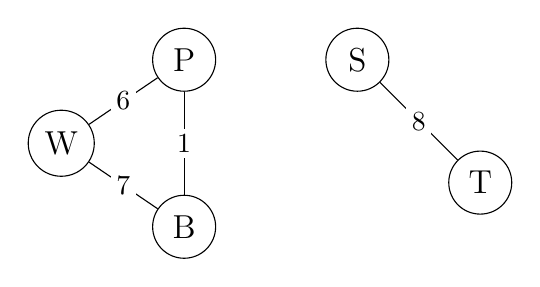
\begin{tikzpicture}[
    node distance={15mm}, 
    main/.style = {draw, circle, font=\large, minimum size=8mm},
    poids/.style = {midway, fill=white, inner sep=2pt}
] 
    % --- Composante de gauche (Triangle W-P-B) ---
    \node[main] (W) {W}; 
    \node[main] (P) [above right of=W, xshift=0.5cm] {P}; 
    \node[main] (B) [below right of=W, xshift=0.5cm] {B}; 

    \draw (W) -- node[poids] {6} (P);
    \draw (W) -- node[poids] {7} (B);
    \draw (P) -- node[poids] {1} (B);

    % --- Composante de droite (Ligne S-T) ---
    \node[main] (S) [right of=P, xshift=0.7cm] {S};
    \node[main] (T) [below right of=S, xshift=0.5cm, yshift=-0.5cm] {T};

    \draw (S) -- node[poids] {8} (T);
    
\end{tikzpicture}
\end{blocvisible}
\end{minipage}
\end{enumerate}
\medskip

On peut adapter un algorithme de parcours de graphe pour déterminer si un graphe est connexe.

On considère la fonction parcours qui permet d'explorer les villes d'un graphe accessibles à partir d'une ville donnée et qui prend en paramètres:
\begin{itemize}
    \item \texttt{graphe}: un dictionnaire représentant le graphe;
    \item \texttt{visitees}: une liste des villes déjà visitées;
    \item \texttt{ville}: la ville actuelle à partir de laquelle on effectue l'exploration.
\end{itemize}

\begin{CodePythontexAlt}[TaillePolice=\large, Largeur=1\linewidth,Centre,Lignes=true,PremLigne=1]{}
def parcours(graphe, visitees, ville):
    """Parcours d'un graphe à partir d'une ville non visitée, 
    en ayant déjà visité un certain nombre de villes."""
    visitees.append(ville)              # Marque la ville comme visitée
    for voisine in graphe[ville].keys():       # Parcourt les voisines de la ville
        if voisine not in visitees:
            # Explore depuis les voisines non visitées
            parcours(graphe, visitees, voisine)  
\end{CodePythontexAlt}

\pagebreak

\begin{enumerate}[resume=monDS]
\item  Expliquer en quoi la fonction \texttt{parcours} est une fonction récursive. (/\getpts{Q22})
\begin{blocvisible}[height=1.5]
    La fonction \texttt{parcours} est une fonction récursive car elle s'appelle elle-même. 
\end{blocvisible}

\medskip

\item Déterminer le contenu des variables \texttt{visitees1} et \texttt{visitees2} après l'exécution des lignes de code données ci-après. (/\getpts{Q23})

\begin{CodePythontexAlt}[TaillePolice=\large, Largeur=1\linewidth,Centre,Lignes=true,PremLigne=1]{}
visitees1 = [ ]
parcours(graphe_airinfo, visitees1, 'W')
visitees2 = [ ]
parcours(graphe_droidevant, visitees2, 'W')
\end{CodePythontexAlt}

\begin{blocvisible}[height=3]
    Après l'exécution de la fonction \texttt{parcours} sur le \texttt{graphe\_airinfo} à partir de la ville \verb|'W'|, la variable \texttt{visitees1} contiendra les villes accessibles depuis \verb|'W'| dans ce graphe, soit \verb|['W', 'P', 'T', 'B', 'S']|.

    Après l'exécution de la fonction \texttt{parcours} sur le \texttt{graphe\_droidevant} à partir de la ville \verb|'W'|, la variable \texttt{visitees2} contiendra les villes accessibles depuis \verb|'W'| dans ce graphe, soit \verb|['W', 'P', 'B']|.
\end{blocvisible}

\medskip
\item Indiquer, parmi les propositions suivantes, laquelle correspond au type de parcours effectué par la fonction parcours (cochez le bonne réponse): (/\getpts{Q24})


\begin{minipage}{0.48\linewidth}
    \begin{itemize}[label=$\square$]
    \item Proposition A\@:  un parcours en largeur;
    \item Proposition B\@: un parcours en grandeur;
    \item Proposition C\@: un parcours en profondeur.
\end{itemize}
\end{minipage}\hfill{}
\begin{minipage}{0.48\linewidth}
    \begin{blocvisible}[height=1.5]
    Réponse: Proposition C\@: un parcours en profondeur (DFS).
    \end{blocvisible}
\end{minipage}



\end{enumerate}


\medskip

On cherche à écrire une fonction \texttt{est\_connexe} qui prend en paramètre un graphe, représenté à l'aide d'un dictionnaire de dictionnaires de voisins, et qui renvoie \texttt{True} si le graphe est connexe, \texttt{False} sinon.

On admet disposer d'une fonction \texttt{ville\_arbitraire} qui renvoie un sommet arbitraire d'un graphe.

Par exemple, \texttt{ville\_arbitraire(graphe\_airinfo)} pourrait renvoyer \verb|'T'| ou n'importe quel autre sommet.

On considère le code de la fonction Python incomplet suivant:

\begin{CodePythontexAlt}[TaillePolice=\large, Largeur=1\linewidth,Centre,Lignes=true,PremLigne=1]{}
def est_connexe(graphe):
    depart = ville_arbitraire(graphe)
    visitees = ...
    parcours(graphe, visitees, depart)  
    return ...
\end{CodePythontexAlt}

\begin{enumerate}[resume=monDS]
    \item Recopier et compléter les lignes 3 et 5 du code de la fonction \texttt{est\_connexe}. On pourra, si nécessaire, ajouter de nouvelles lignes. (/\getpts{Q25})

\begin{blocvisible}[height=3.5]
\begin{CodePythontexAlt}[TaillePolice=\large, Largeur=1\linewidth,Centre,Lignes=true,PremLigne=1]{}
def est_connexe(graphe):
    depart = ville_arbitraire(graphe)
    visitees = [ ]
    parcours(graphe, visitees, depart)
    return len(visitees) == len(graphe)
\end{CodePythontexAlt}
\end{blocvisible}

\end{enumerate}
\pagebreak


On considère maintenant le code de la fonction, donné ci-après, \texttt{mystere}, qui prend en paramètres:

\begin{itemize}
    \item \texttt{graphe}, un dictionnaire représentant un graphe;
    \item \texttt{ville}, une clé du dictionnaire graphe représentant une ville de départ;
    \item \texttt{chemin}, une liste de clés représentant les villes déjà visitées sur le chemin parcouru depuis la ville de départ;
    \item \texttt{cout}, un entier représentant une distance parcourue depuis la ville de départ;
    \item \texttt{arrivee}, une clé du dictionnaire graphe représentant une ville d'arrivée.
\end{itemize}

\begin{CodePythontexAlt}[TaillePolice=\large, Largeur=1\linewidth,Centre,Lignes=true,PremLigne=1]{}
def mystere(graphe, ville, chemin, cout, arrivee):
    # Ajoute la ville actuelle au chemin 
    chemin = chemin + [ville]
    if ville == arrivee:
        # Affiche le chemin et son coût total 
        print(chemin, cout) 
    # Parcourt les villes voisines et leurs poids 
    for voisine, poids in graphe[ville].items():
        # Vérifie que la ville n'est pas déjà visitée 
        if voisine not in chemin: 
            mystere(graphe, voisine, chemin, cout + poids, arrivee)
        \end{CodePythontexAlt}

\begin{enumerate}[resume=monDS]
    \item Déterminer les affichages produits lors de l'exécution de l'appel suivant: (/\getpts{Q26})
\begin{CodePythontexAlt}[TaillePolice=\large, Largeur=1\linewidth,Centre,Lignes=true,PremLigne=1]{}
mystere(graphe_airinfo, 'W', [ ], 0, 'B')
\end{CodePythontexAlt}
\begin{blocvisible}[height=3]
    Les affichages produits lors de l'exécution de l'appel suivant:
\begin{CodePythontexAlt}[TaillePolice=\large, Largeur=1\linewidth,Centre,Lignes=true,PremLigne=1]{}
['W', 'P', 'T', 'B'] 25
['W', 'P', 'S', 'T', 'B'] 40
\end{CodePythontexAlt}
\end{blocvisible}

\medskip

\item Expliquer, de manière générale, ce que réalise l'appel \texttt{mystere(graphe, ville, [ ], 0, arrivee)} pour un graphe \texttt{graphe} et deux villes \texttt{ville} et \texttt{arrivee}. (/\getpts{Q27})
\begin{blocvisible}[height=5]
    L'appel \texttt{mystere(graphe, ville, [ ], 0, arrivee)} réalise une recherche de tous les chemins possibles entre la ville de départ (\texttt{ville}) et la ville d'arrivée (\texttt{arrivee}) dans le graphe \texttt{graphe}. 

    La fonction utilise une approche récursive pour explorer les différentes routes possibles. À chaque étape, elle ajoute la ville actuelle au chemin parcouru et met à jour le coût total en ajoutant le poids de l'arête correspondante. 

    Lorsque la fonction atteint la ville d'arrivée, elle affiche le chemin parcouru ainsi que son coût total. En explorant toutes les voies possibles, elle permet de trouver tous les chemins entre les deux villes et leurs coûts associés.
\end{blocvisible}


\end{enumerate}
            
